\subsection{Levantamento de Hipóteses e Oportunidades de Solução}

A primeira atividade realizada consistiu no levantamento de hipóteses sobre o produto, formuladas a partir de suposições dos \textit{stakeholders}, motivadas por diversos fatores, como conhecimento de negócio, estado do mercado e concorrência. Dessa forma, inicialmente, os colaboradores foram instruídos a compartilhar suas percepções, que seriam discutidas para que uma delas fosse selecionada e validada por meio de um experimento.

Todas as hipóteses levantadas foram documentadas na plataforma Notion \cite{notion}, onde foram registradas suas motivações, objetivos e demais informações relevantes, com o propósito de armazenar o conhecimento gerado pelo processo e criar um repositório compartilhado dentro da empresa (ver Apêndice \ref{apdx:notion}). 

Após a discussão, uma hipótese foi escolhida, relacionada à subutilização de uma funcionalidade específica da plataforma. O produto permite que docentes criem listas de exercícios para aplicação posterior com os estudantes. Durante esse processo, o usuário seleciona manualmente as questões e, para facilitar essa busca, o sistema oferece uma série de filtros que ajudam a encontrar os itens mais adequados às necessidades do professor. A funcionalidade pode ser melhor compreendida na Figura \ref{fig:selecao-questoes-tratamento} (barra de filtros à esquerda).

A funcionalidade subutilizada refere-se a um filtro por nível de dificuldade da questão. Um dos colaboradores identificou, a partir de dados quantitativos disponibilizados pelo Mixpanel \cite{mixpanel2024}, que esse era o filtro menos utilizado entre todas as categorias. No entanto, essa informação contrariava as expectativas da equipe, pois a inclusão desse filtro havia sido amplamente solicitada pelos professores durante processos de \textit{feedback} sobre a plataforma.

Além disso, a categorização das questões exige um esforço adicional para além das alterações no código-fonte, uma vez que o time editorial realiza manualmente essa classificação, questão por questão. Assim, a empresa esperava que o uso da funcionalidade fosse proporcional ao esforço investido em sua implementação.

Diante dessa percepção, o colaborador levantou a hipótese de que a baixa adoção do filtro poderia estar relacionada à sua posição na interface, já que ele se encontrava no final da lista. Especulou-se que, para usuários com telas menores, o filtro poderia ser menos acessível. Como solução, propôs-se mover o filtro para uma posição mais destacada e observar se essa alteração influenciaria o comportamento dos usuários, aumentando sua utilização. Por estar alinhada aos objetivos estratégicos da equipe e envolver baixa complexidade de desenvolvimento (algo necessário, dado o cronograma limitado deste trabalho), essa foi a hipótese escolhida para o experimento.


\begin{figure}
    \centering
    \caption{Versão de Controle do Produto Analisado}
    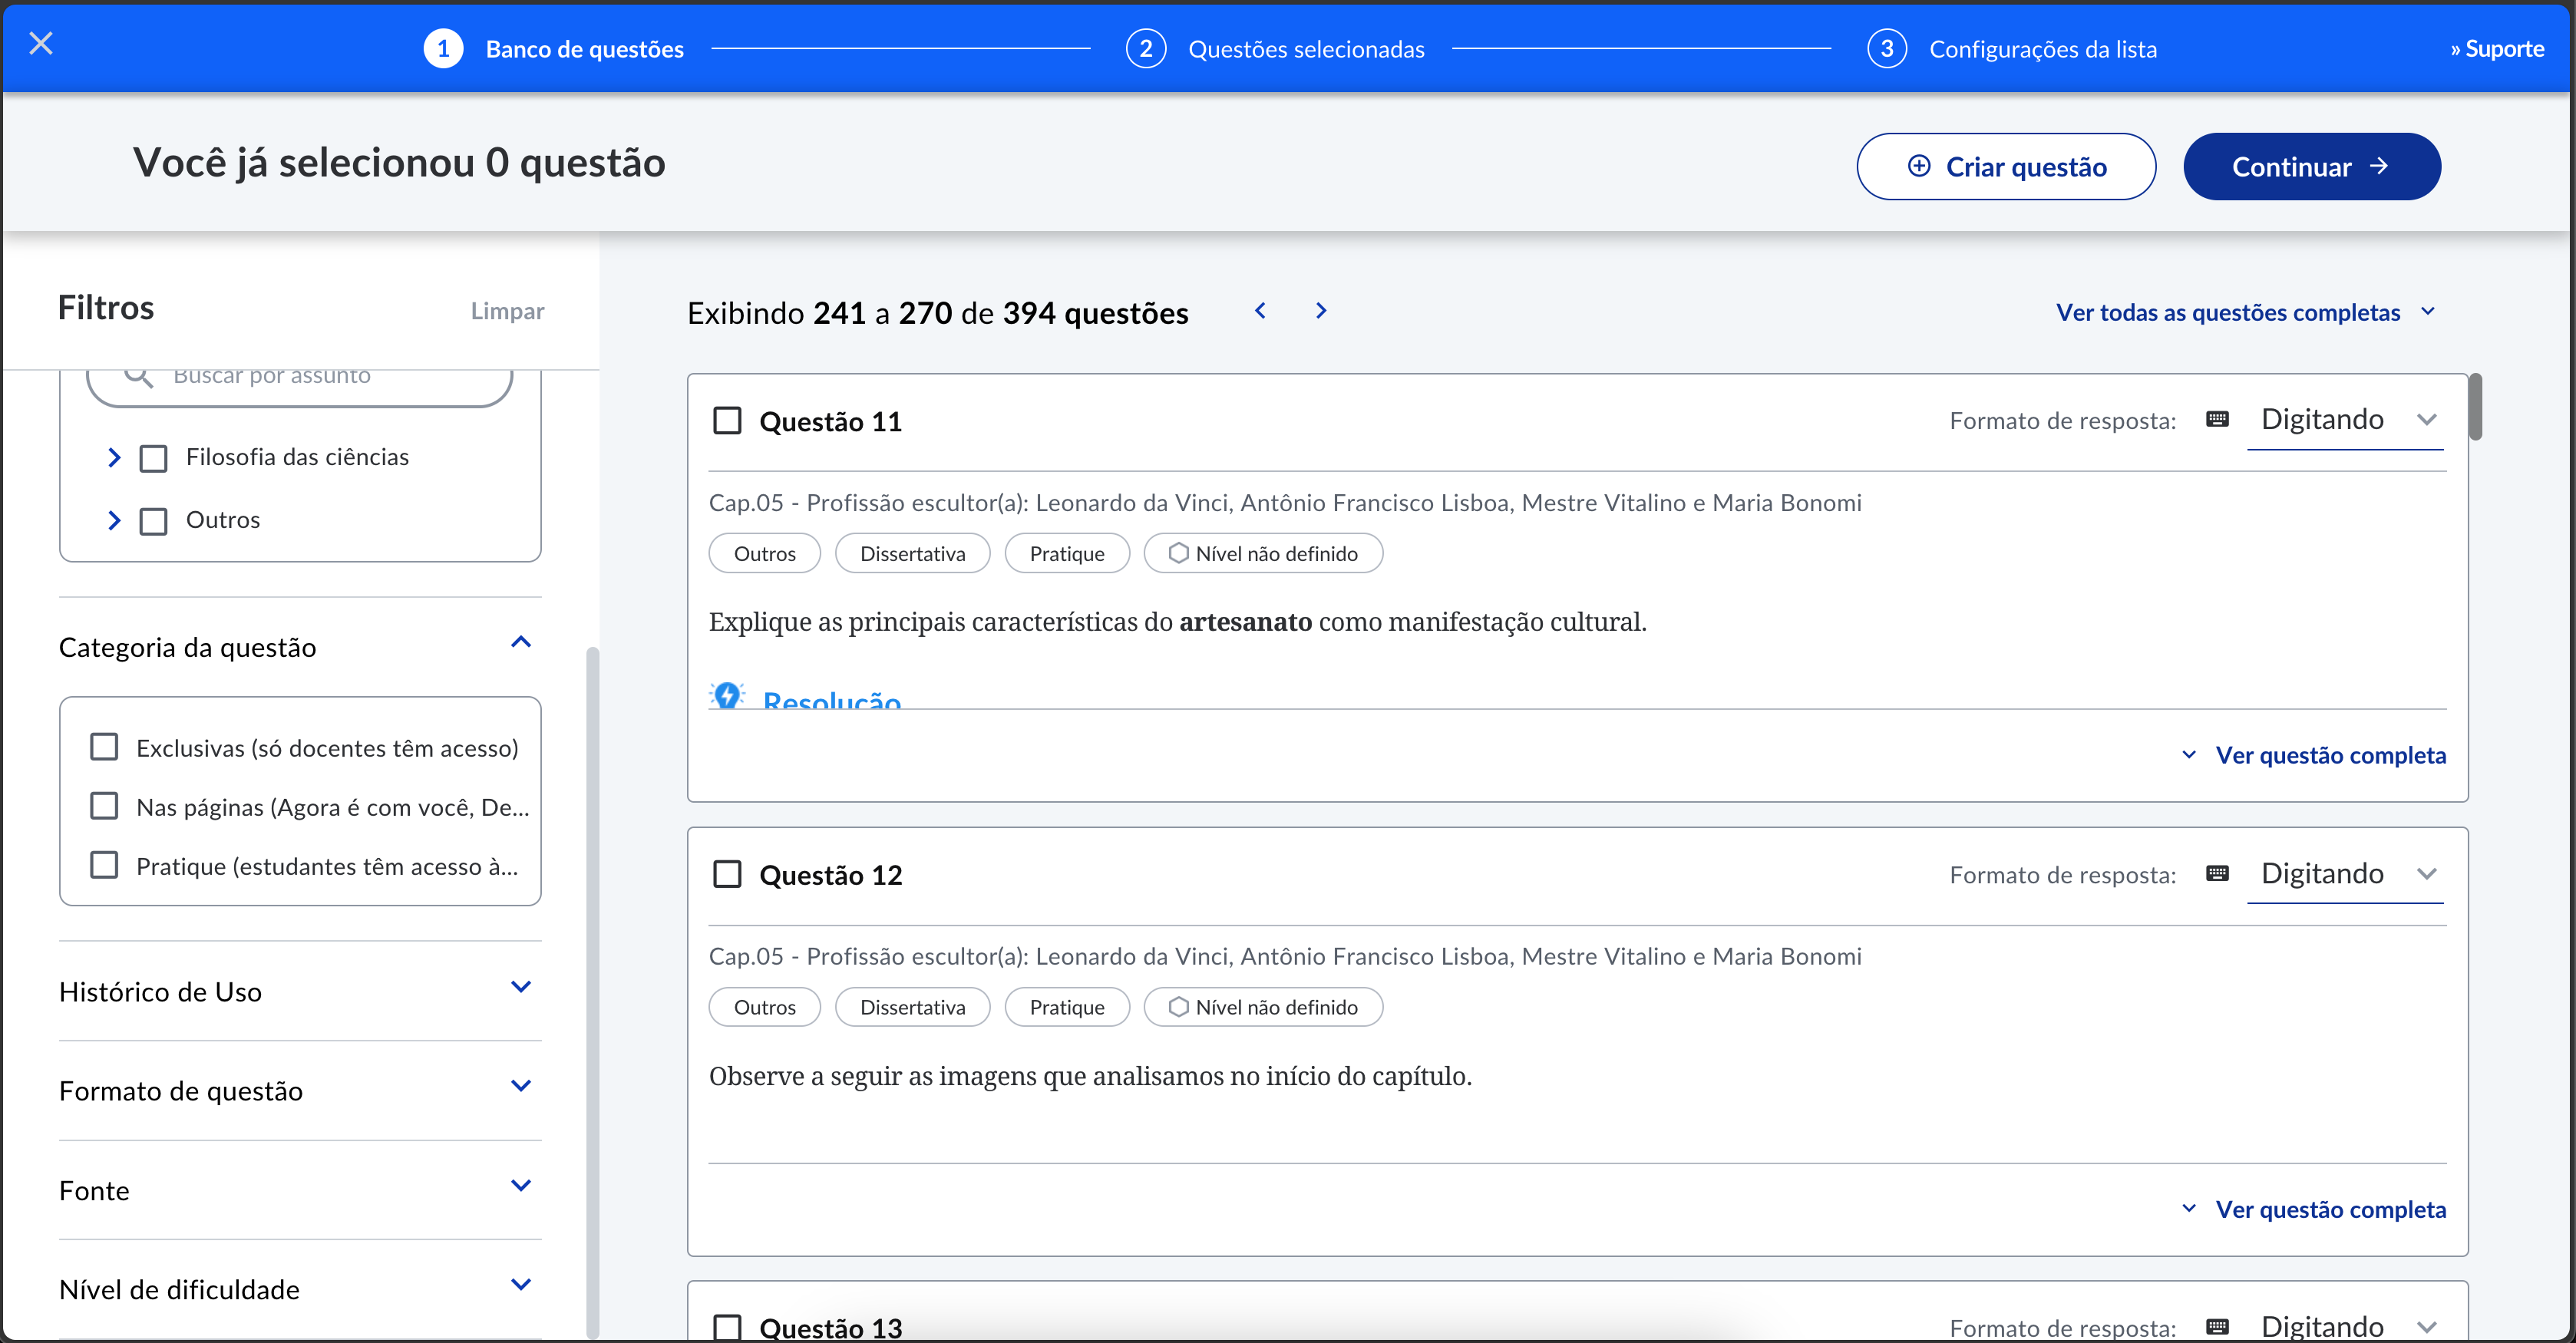
\includegraphics[width=1\linewidth]{figuras/selecao-questoes-controle.png}
    \begin{center}
        \text{Fonte: Autor}
    \end{center}
    \label{fig:selecao-questoes-tratamento}
\end{figure}
